% ══════════════════════════════════════════════════════════════════════════════
%  CS495-Capstone-Poster.tex
%  CS495 -- Data Science Project Practicum
%  Capstone Poster -- Bellevue College
%  Size:  36" x 48" portrait
%  Build: pdflatex CS495-Capstone-Poster.tex      (run twice)
%
%  Based on CS495-Poster-Template.tex (BC brand chrome).
%  Embedded figures retain the project's navy / skyblue palette.
% ══════════════════════════════════════════════════════════════════════════════

\documentclass[a0,portrait]{a0poster}

% ── Override paper to 36" x 48" portrait ──────────────────────────────────────
\setlength{\paperwidth}{36in}
\setlength{\paperheight}{48in}
\special{papersize=36in,48in}

% ---------- Packages ----------
\usepackage[utf8]{inputenc}
\usepackage[T1]{fontenc}
\usepackage[english]{babel}
\usepackage{graphicx}
\graphicspath{{./}{../../assets/figures/}{../../assets/branding/}}
\usepackage{amsmath,amssymb}
\usepackage{booktabs}
\usepackage{array}
\usepackage{multicol}
\usepackage{xcolor}
\usepackage{enumitem}
\usepackage{tcolorbox}
\usepackage{tikz}
\usetikzlibrary{positioning, arrows.meta, calc}
\usepackage{ragged2e}
\usepackage{anyfontsize}
\usepackage{qrcode}
\tcbuselibrary{skins,breakable}

% ── Page geometry override for 36"x48" ────────────────────────────────────────
\setlength{\hoffset}{-1in}
\setlength{\voffset}{-1in}
\setlength{\oddsidemargin}{2cm}
\setlength{\evensidemargin}{2cm}
\setlength{\topmargin}{2cm}
\setlength{\headheight}{0pt}
\setlength{\headsep}{0pt}
\setlength{\topskip}{0pt}
\setlength{\textwidth}{\dimexpr\paperwidth-4cm\relax}
\setlength{\textheight}{\dimexpr\paperheight-4cm\relax}

% ---------- Bellevue College Brand Colors ----------
\definecolor{BCBlue}{HTML}{003D79}        % Brutus Blue   (primary)
\definecolor{BCSilver}{HTML}{A7A9AC}      % Bulldog Silver (primary)
\definecolor{BCRed}{HTML}{C4122F}         % Fall Maple Red (accent)
\definecolor{BCLightBlue}{HTML}{E6EEF7}   % Soft tinted background
\definecolor{BCDarkBlue}{HTML}{002851}    % Deeper variant
\definecolor{BCInk}{HTML}{1A1A1A}         % Body text

% ---------- Layout ----------
\setlength{\parindent}{0pt}
\setlength{\parskip}{0.3em}
\setlength{\columnsep}{2.0cm}
\setlength{\columnseprule}{0pt}

% ---------- Block container (BC brand chrome) ----------
\newtcolorbox{posterblock}[1]{
    enhanced, breakable,
    colback=white, colframe=BCSilver,
    boxrule=0.8pt, arc=6pt,
    left=14pt, right=14pt, top=6pt, bottom=10pt,
    fonttitle=\bfseries\Large,
    title={#1},
    coltitle=white,
    colbacktitle=BCBlue,
    attach boxed title to top left={xshift=0mm, yshift=0mm},
    boxed title style={
        colback=BCBlue, colframe=BCBlue,
        sharp corners, boxrule=0pt,
        left=14pt, right=18pt, top=6pt, bottom=6pt,
    },
    title filled=true,
    before skip=10pt, after skip=10pt,
    overlay unbroken and first={
        \fill[BCRed] (frame.north west) rectangle ([xshift=12pt]frame.north west|-title.south);
    },
}

% ---------- Inline tinted callout (for equations / key facts) ----------
\newtcolorbox{callout}{
    colback=BCLightBlue, colframe=BCLightBlue,
    arc=4pt, left=14pt, right=14pt, top=10pt, bottom=10pt,
    boxrule=0pt,
}

% ══════════════════════════════════════════════════════════════════════════════
\begin{document}

% ══════════════════════════════════════════════════════════════════════════════
%  TITLE BANNER
% ══════════════════════════════════════════════════════════════════════════════
\noindent

\begin{tikzpicture}[remember picture]
  \fill[BCLightBlue] (0,0) rectangle (\textwidth, 11cm);
  \fill[BCRed]  (0,0) rectangle (\textwidth, 0.6cm);

  % Bellevue College logo on the left
  \node[anchor=west, inner sep=0pt] at (1cm, 6cm) {
    \IfFileExists{BellevueCollegeLogoHorzClr.png}{%
      \includegraphics[height=7cm]{BellevueCollegeLogoHorzClr.png}%
    }{%
      \colorbox{BCDarkBlue}{\parbox[c][7cm][c]{22cm}{\centering\bfseries
        \color{BCBlue}\fontsize{50}{60}\selectfont Bellevue College}}%
    }
  };

  % Title text on the right --- FULL width (the headline stays prominent)
  \node[anchor=west, inner sep=0pt, text width=\textwidth-32cm, align=left]
       at (32cm, 8.2cm) {%
    \color{BCDarkBlue}\fontsize{60}{72}\selectfont\bfseries
    Mathematical and Empirical Models in Agreement
  };

  % Subtitle / author / course --- narrowed by ~7 cm to make room for the QR
  \node[anchor=west, inner sep=0pt, text width=\textwidth-39cm, align=left]
       at (32cm, 5.0cm) {%
    \color{BCDarkBlue}\fontsize{36}{44}\selectfont
    Cross-Validating CRR Binomial Pricing and Machine Learning\\
    for Crowd Mispricing Detection in Equity Options
  };
  \node[anchor=west, inner sep=0pt, text width=\textwidth-39cm, align=left]
       at (32cm, 2.7cm) {%
    \color{BCDarkBlue}\fontsize{30}{36}\selectfont
    \textbf{Author:} DeWayne Dantzler \quad\textbar\quad
    \textbf{Faculty Advisor:} Dr.~Pedro Albuquerque
  };
  \node[anchor=west, inner sep=0pt, text width=\textwidth-39cm, align=left]
       at (32cm, 1.2cm) {%
    \color{BCDarkBlue}\fontsize{24}{30}\selectfont\itshape
    CS\,495 -- Data Science Project Practicum \;\textbullet\;
    Bellevue College \;\textbullet\; Spring 2026
  };

  % QR code on the far right side of the banner, vertically centered on the subtitle block
  \node[anchor=east] at (\textwidth - 1cm, 4.5cm)
       {\fbox{\qrcode[height=5cm]{https://github.com/dantzlerdc/CS495-Deep-Scholar}}};
\end{tikzpicture}

\vspace{2cm}

% ══════════════════════════════════════════════════════════════════════════════
%  THREE-COLUMN BODY
% ══════════════════════════════════════════════════════════════════════════════
\RaggedRight
\normalsize

\begin{multicols}{3}

% ──────────────────────────────────────────────────────────────────────────────
%  LEFT COLUMN
% ──────────────────────────────────────────────────────────────────────────────

\begin{posterblock}{Abstract}
This project addresses a foundational question in quantitative finance:
when an options pricing model produces a theoretical fair value that
diverges from the observed market premium, is that divergence large
enough --- and reliable enough --- to justify a trade? A Cox--Ross--%
Rubinstein (CRR) American binomial option pricer is built in vectorized
Python and validated against a live AMD option chain from Fidelity
(April 2026). Its mispricing-edge signal is then cross-validated against
an independent XGBoost ITM/OTM probability classifier trained on
101{,}535 historical AAPL contracts. The two layers agree strongly in
the herding regime (Pearson correlation $r=0.413$,
$p=2.4\times10^{-10}$) and not at all in the normal regime ($r\approx0$).
A regime-conditioned Kelly Criterion framework converts the
cross-validated edge into risk-controlled capital allocation.

\vspace{0.4em}
\textbf{Keywords:} CRR binomial pricing, options mispricing, XGBoost,
Kelly Criterion, behavioral finance, EMH, herding regime.
\end{posterblock}

\begin{posterblock}{Introduction \& Motivation}
Options markets aggregate beliefs into prices much like prediction
markets do, but behavioral forces --- herding around round strikes,
implied-volatility overpricing driven by fear, and systematic skew in
out-of-the-money puts --- distort prices in predictable ways. The gap
between a pricing model's theoretical fair value and the observed
market premium is potentially exploitable by a disciplined, model-driven
strategy, but only if the divergence is large enough, reliable enough,
and detectable by independent methods.

\vspace{0.5em}
\textbf{Research Questions}
\begin{itemize}[leftmargin=1.4em,itemsep=4pt,topsep=4pt]
  \item Do CRR model prices predict whether an equity option expires
        in-the-money or out-of-the-money?
  \item Does cross-validation between CRR (math) and an ML classifier
        detect exploitable pricing \emph{edge}?
  \item Does regime-conditioned Kelly sizing convert that edge into
        positive expected value?
\end{itemize}

\vspace{0.3em}
\textbf{Objectives}
\begin{itemize}[leftmargin=1.4em,itemsep=4pt,topsep=4pt]
  \item Implement the CRR American binomial lattice (no dividends) in
        vectorized Python at $N=100$ steps.
  \item Validate pricing accuracy against AMD market premiums within
        $\pm 5\%$ error.
  \item Train an XGBoost ITM/OTM classifier on engineered features
        \emph{without} using IV as an input (independence from L1).
  \item Apply Kelly Criterion (full / half / quarter) for
        risk-controlled position sizing.
\end{itemize}
\end{posterblock}

\begin{posterblock}{Data Description}
Two datasets are used --- a large historical training corpus for the
ML layer and a small live chain for end-to-end validation.

\vspace{0.6em}
\renewcommand{\arraystretch}{1.35}
\begin{tabular}{@{}p{0.34\linewidth}p{0.60\linewidth}@{}}
\toprule
\textbf{Attribute} & \textbf{Description} \\
\midrule
Training source & AAPL options, Kaggle (2016--2020) \\
Sample size     & 101{,}535 contracts (walk-forward 60/20/20) \\
Live source     & AMD chain, Fidelity (April 2026) \\
Live tickets    & 4 trade tickets at $\sigma \approx 64\%$ \\
Features        & $S$, $K$, $T$, $r$, IV, RV30, bid/ask, OI, volume \\
Time range      & 2016-01 -- 2026-04 \\
Missing data    & None for engineered features \\
\bottomrule
\end{tabular}
\end{posterblock}

\begin{posterblock}{Exploratory Data Analysis}
Plotting each contract's Layer-1 edge against its Layer-2 edge reveals
the central empirical finding of the project: agreement between the
two independent models concentrates in the \emph{herding} regime
(red), not in the \emph{normal} regime (gray).

\vspace{0.4em}
\begin{center}
  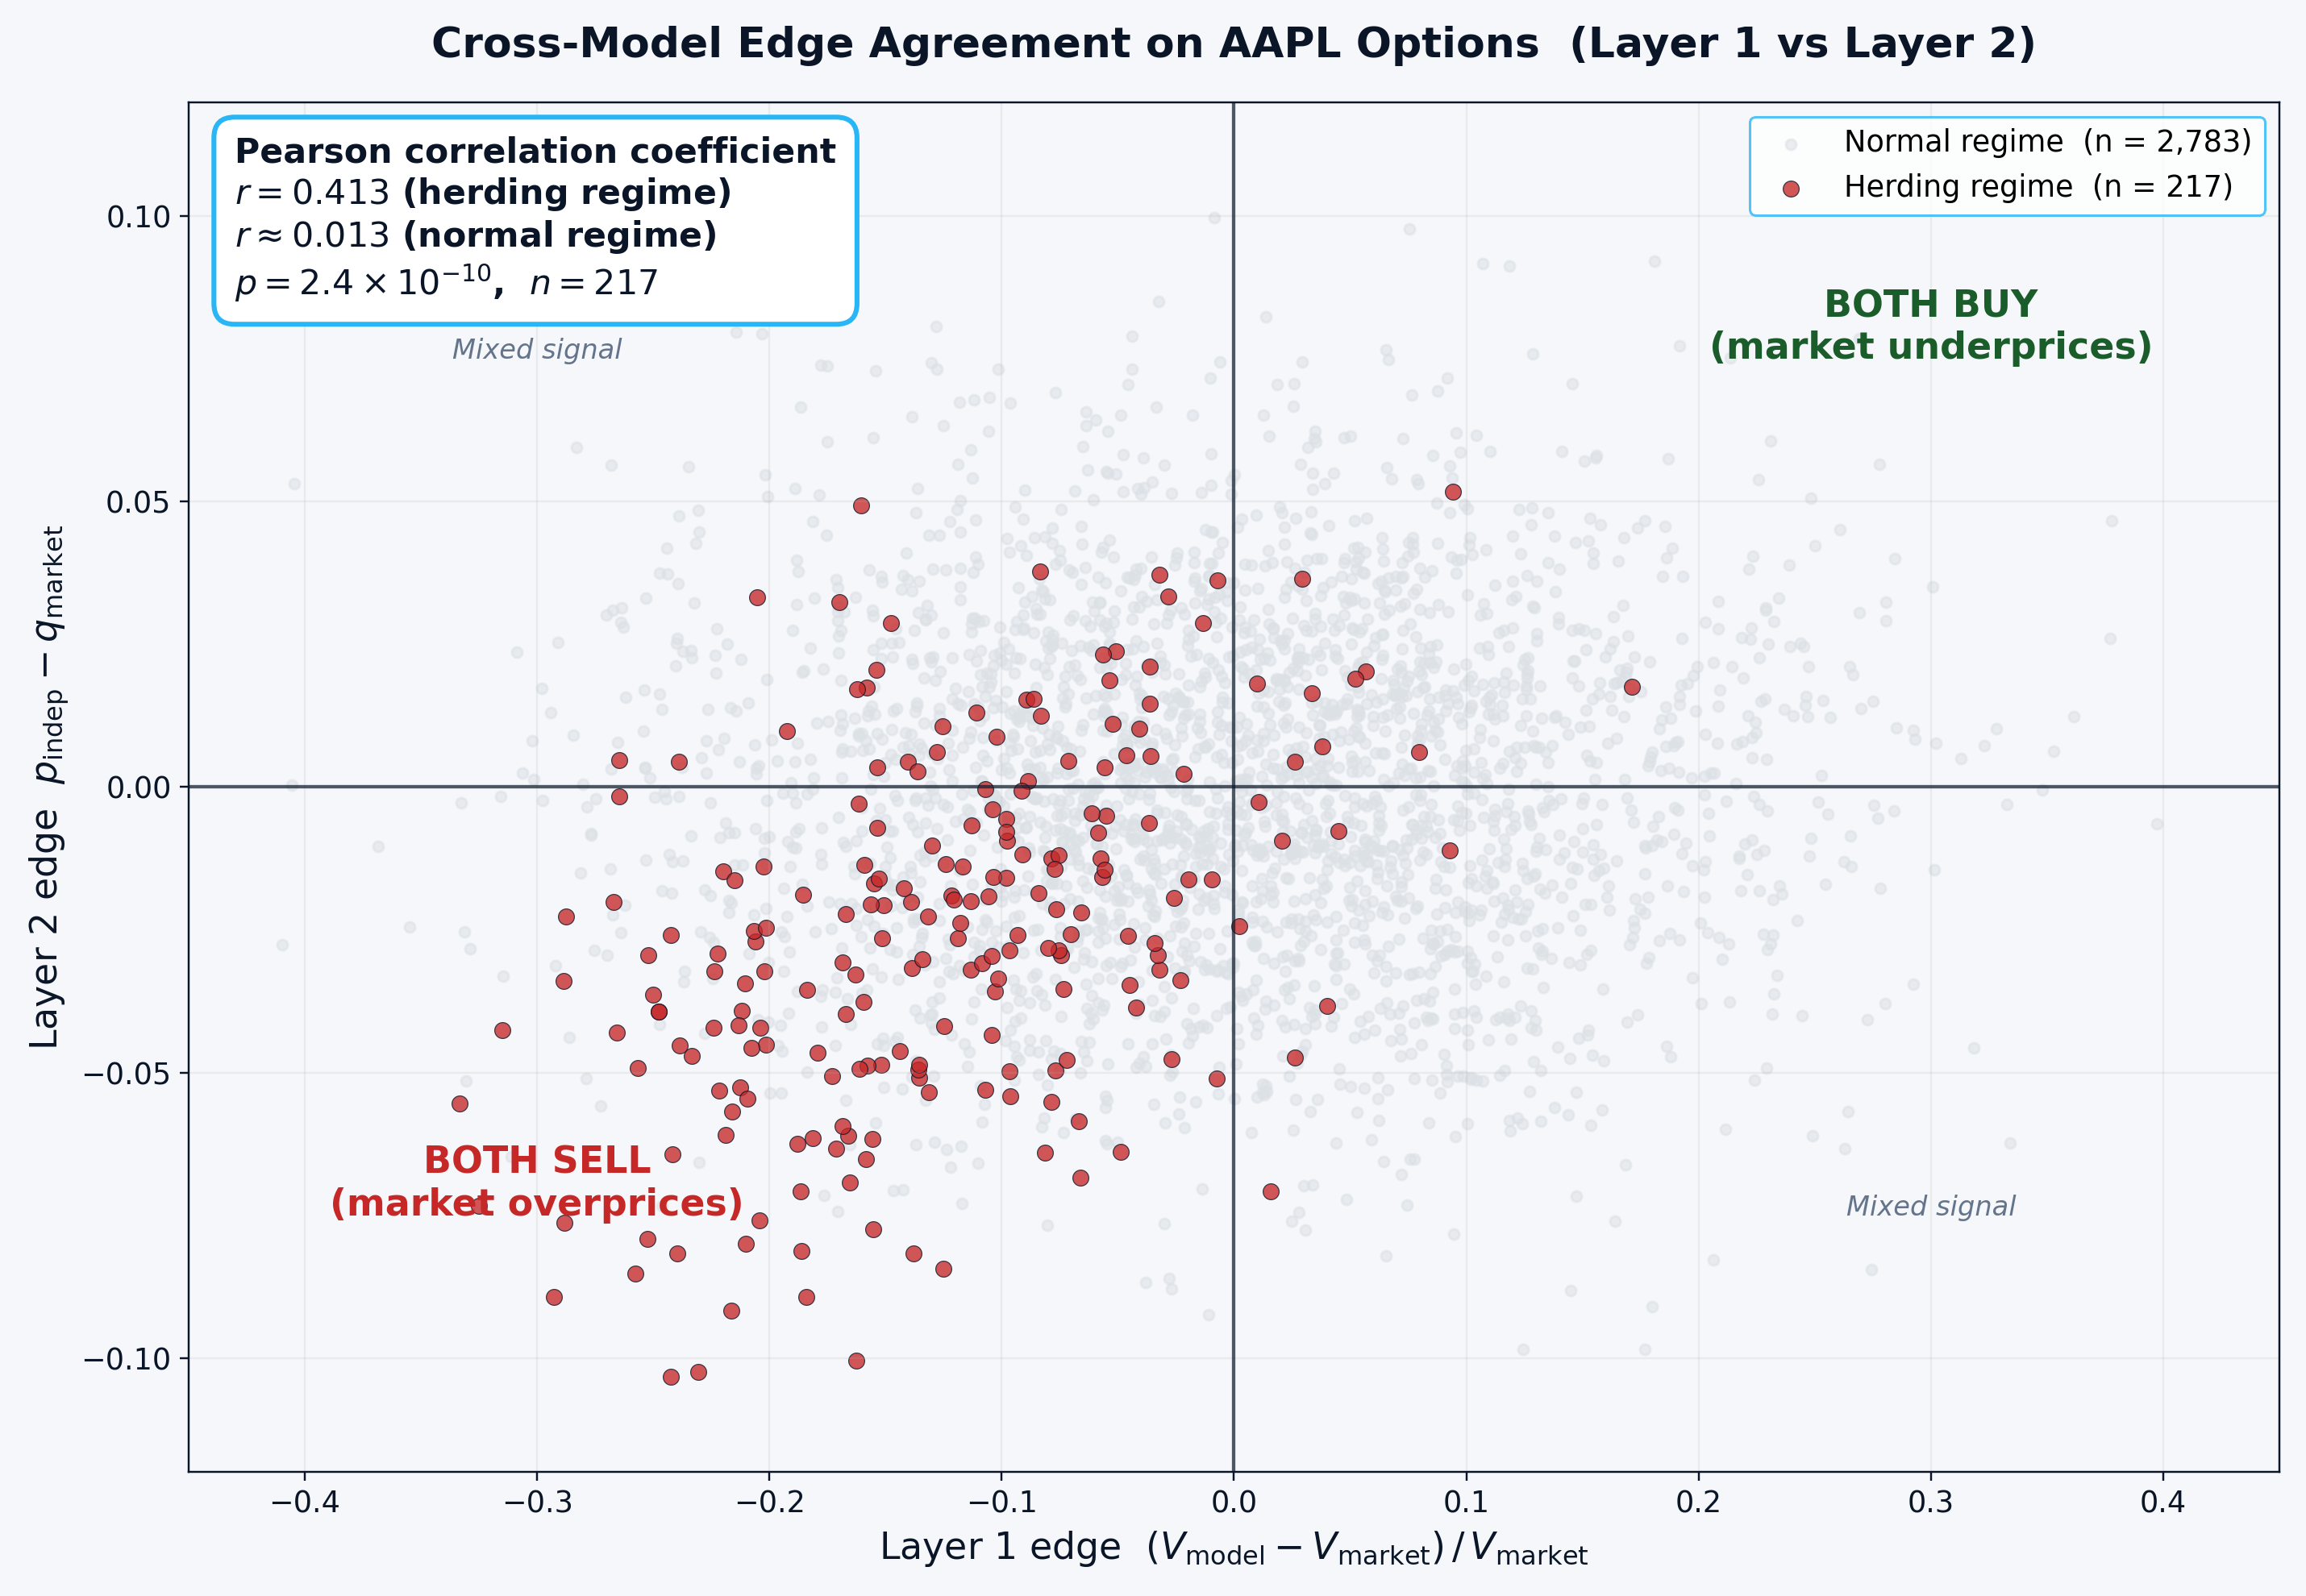
\includegraphics[width=0.86\linewidth,keepaspectratio]
    {Poster-Hero-Scatter.png}
\end{center}

\vspace{0.3em}
\textbf{Key pattern:} Pearson correlation coefficient
$r=0.413$ in herding regime (red cluster in Q3 -- both layers say
SELL) versus $r\approx0$ in normal regime (gray cloud).
This is the empirical fingerprint of \emph{Samuelson macro-inefficiency}
--- markets are micro-efficient on average but exhibit aggregate bias
under coordinated behavioral demand.
\end{posterblock}

% ──────────────────────────────────────────────────────────────────────────────
\columnbreak
%  CENTER COLUMN
% ──────────────────────────────────────────────────────────────────────────────

\begin{posterblock}{Methodology}
A three-layer pipeline runs CRR and ML independently, then merges their
edge signals.

\vspace{0.6em}
\begin{center}
\begin{tikzpicture}[node distance=0.5cm,
    box/.style={rounded corners=4pt, text=white,
                font=\bfseries\large, minimum width=16cm,
                minimum height=1.5cm, align=left, inner xsep=12pt}]
  \node[box, fill=BCBlue] (l1)
    {\textcolor{BCLightBlue}{Layer 1\ \ }CRR Binomial Pricer  $\;\to\;$ edge$_{L1}$};
  \node[box, fill=BCDarkBlue, below=of l1] (l2)
    {\textcolor{BCLightBlue}{Layer 2\ \ }XGBoost ITM/OTM Classifier  $\;\to\;$ edge$_{L2}$};
  \node[box, fill=BCRed,      below=of l2] (l3)
    {\textcolor{BCLightBlue}{Layer 3\ \ }Regime-Conditioned Kelly Sizing};
  \draw[-{Stealth[length=8pt]}, BCBlue,    line width=1.6pt] (l1.south) -- (l2.north);
  \draw[-{Stealth[length=8pt]}, BCDarkBlue,line width=1.6pt] (l2.south) -- (l3.north);
\end{tikzpicture}
\end{center}

\vspace{0.4em}
\textbf{Techniques used}
\begin{itemize}[leftmargin=1.4em,itemsep=4pt,topsep=4pt]
  \item Vectorized recombining lattice in NumPy ($N{=}50$ to $100$ steps).
  \item Backward induction with American early-exercise check at each node.
  \item Greeks via centered finite differences.
  \item XGBoost trained on engineered features only ($\sigma$ input is
        RV30, never IV --- no leakage from L1).
  \item Platt scaling calibration; Brier-score validation.
  \item Walk-forward 60/20/20 split; zero look-ahead bias.
\end{itemize}
\end{posterblock}

\begin{posterblock}{Model \& Analysis}
The CRR lattice is built from no-arbitrage relations and solved by
backward induction with American early-exercise:

\vspace{0.3em}
\begin{callout}
\centering\large
$\displaystyle u = e^{\sigma\sqrt{\Delta t}}, \quad d = 1/u, \quad
 p^{*} = \dfrac{e^{r\Delta t}-d}{u-d}$
\\[0.3em]
$\displaystyle V_{\text{node}} = \max\!\Bigl(\text{intrinsic},\ \
 e^{-r\Delta t}\bigl(p^{*}V_{u} + (1-p^{*})V_{d}\bigr)\Bigr)$
\end{callout}

\vspace{0.3em}
The mispricing edge per contract is the signed percentage deviation
between model and market premium, and the Kelly Criterion sets the
fraction of capital to commit:

\vspace{0.3em}
\begin{callout}
\centering\large
$\displaystyle \text{edge} = \frac{V_{\text{model}} - V_{\text{market}}}
                                       {V_{\text{market}}}, \quad
 f^{*} = \frac{p\!\cdot\! b - q}{b}$
\end{callout}

\vspace{0.5em}
\textbf{Training / validation setup}
\begin{itemize}[leftmargin=1.4em,itemsep=4pt,topsep=4pt]
  \item Train / val / test: 60 / 20 / 20 walk-forward by quote date.
  \item Cross-validation: 5-fold within training window.
  \item Hyperparameter tuning: Bayesian search over XGBoost
        (depth, $\eta$, $n_{\text{trees}}$).
  \item Regime split: IV/RV$_{30}$ ratio
        ($>1.10$ herding, $<0.90$ normal, between = transition).
\end{itemize}
\end{posterblock}

\begin{posterblock}{Forward + Backward Pass}
\textit{Real AAPL put, 2020-03-16, herding regime
($S=\$241.47$, $K=\$240$, DTE $=18$d).}

\vspace{0.4em}
\begin{center}
  \textbf{\large Forward Pass}\\[0.15em]
  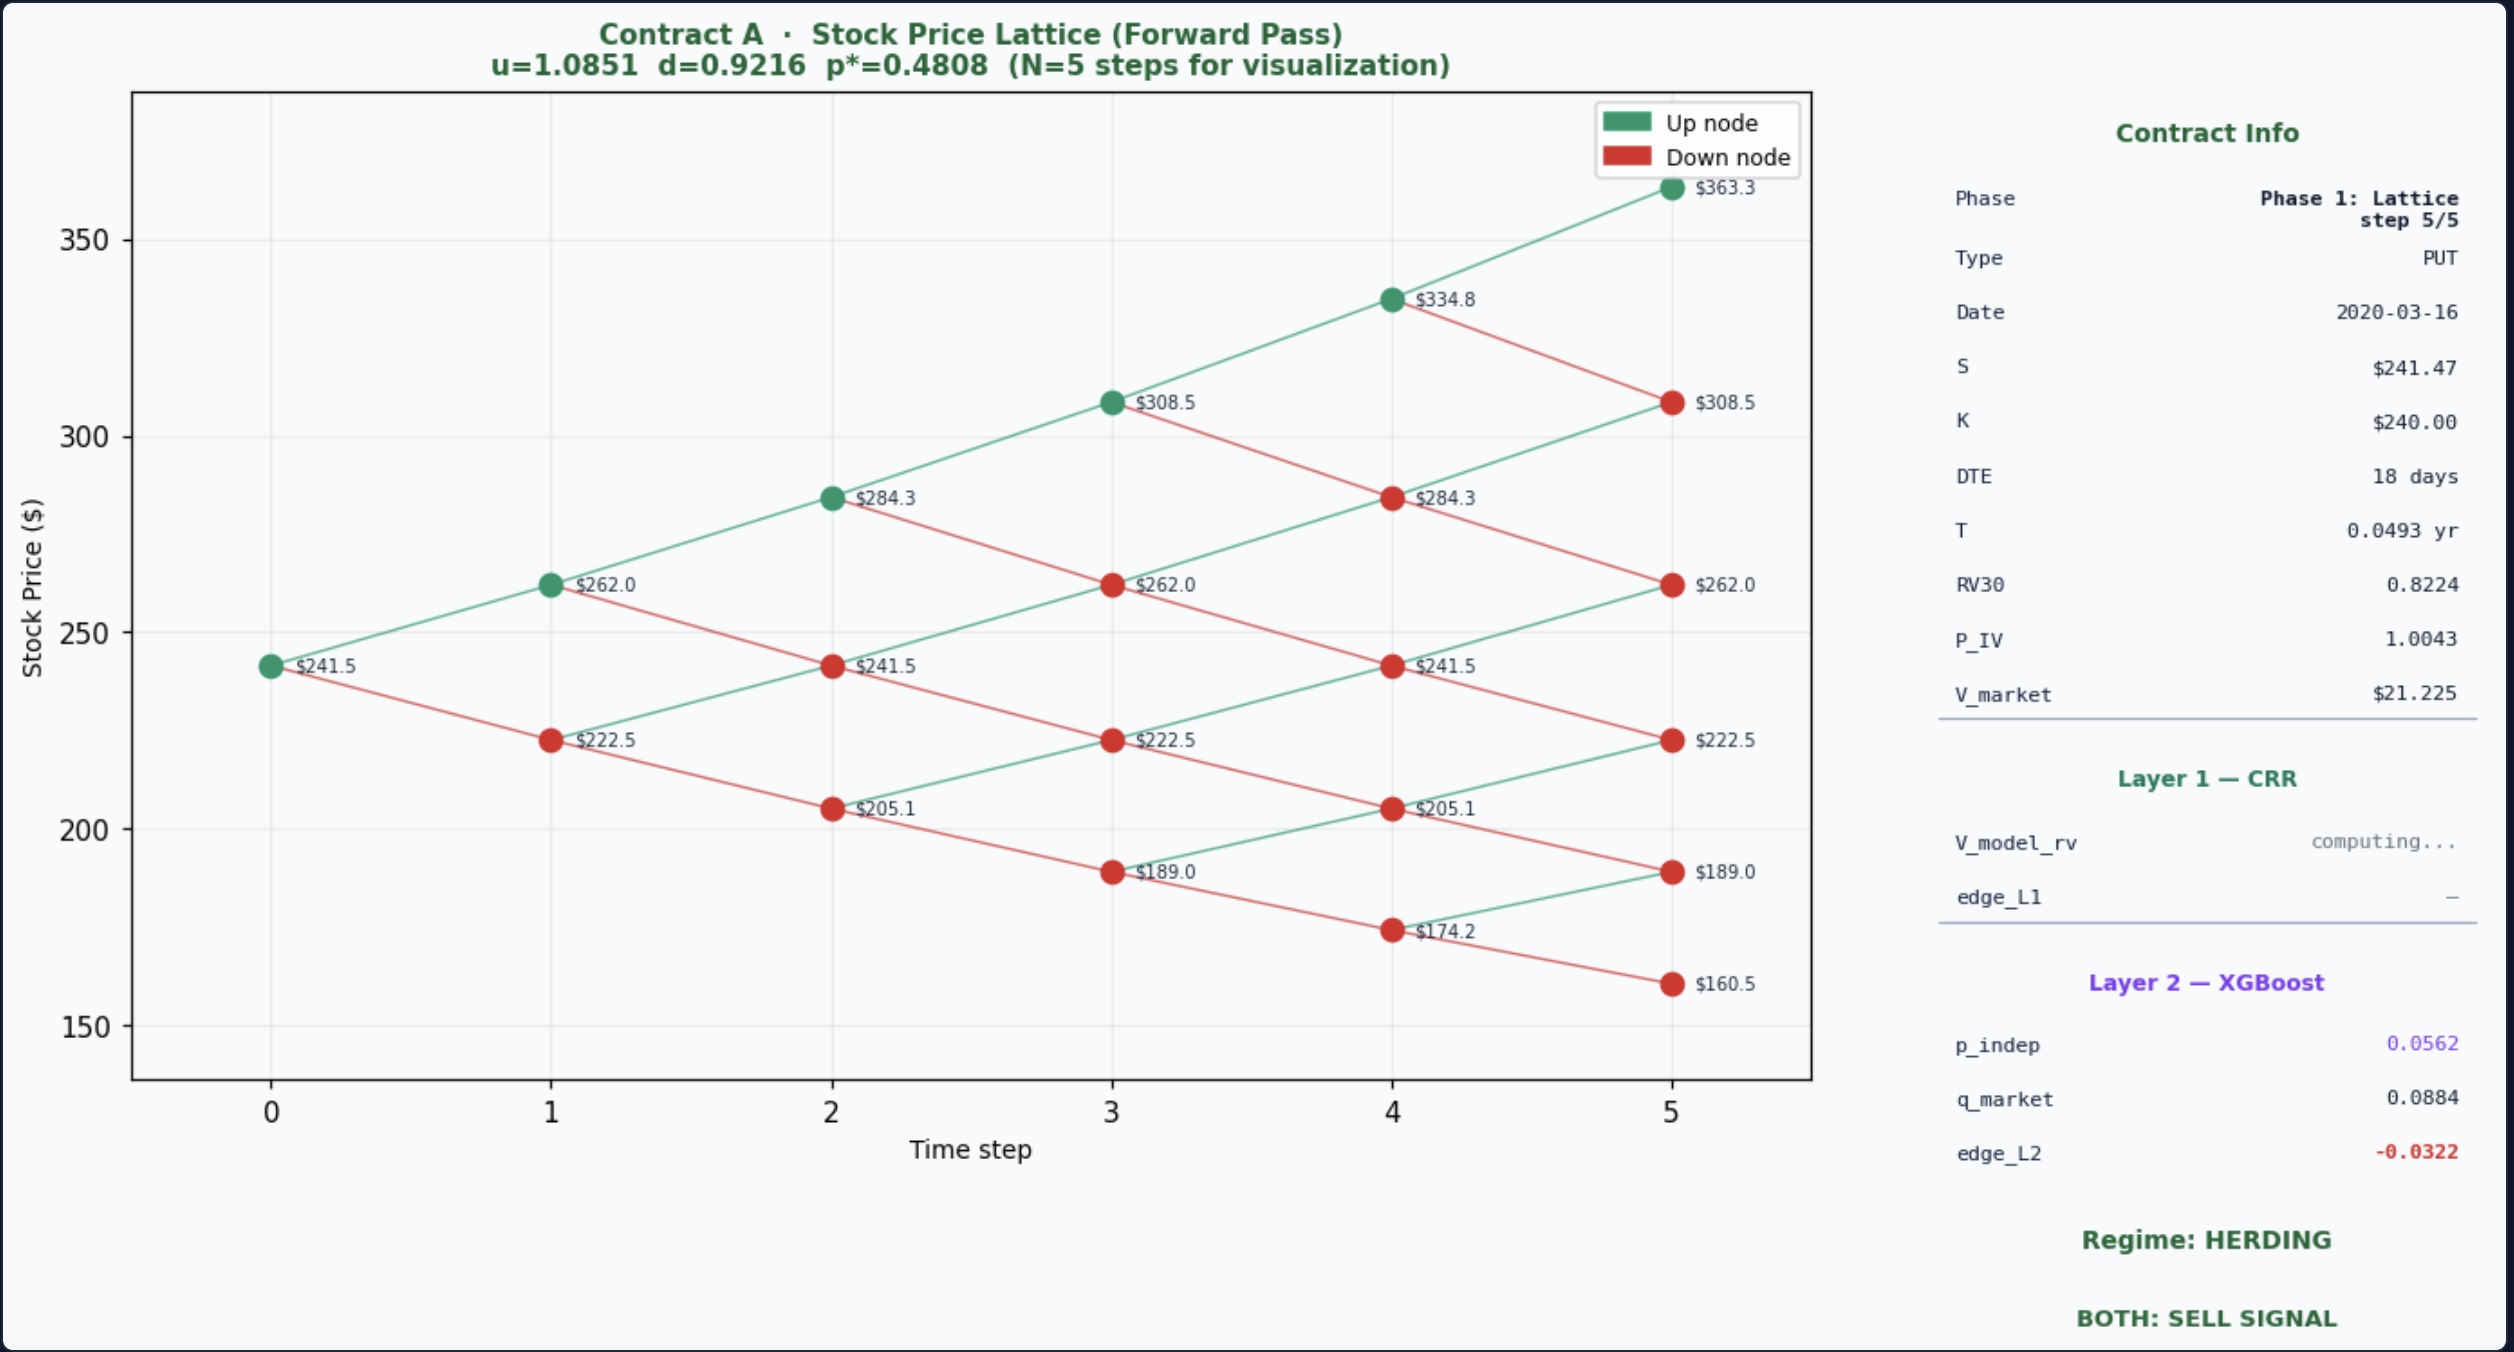
\includegraphics[width=0.62\linewidth,keepaspectratio]
    {Poster-Forward-Pass.png}
\end{center}

\vspace{0.3em}
\begin{center}
  \textbf{\large Backward Induction}\\[0.15em]
  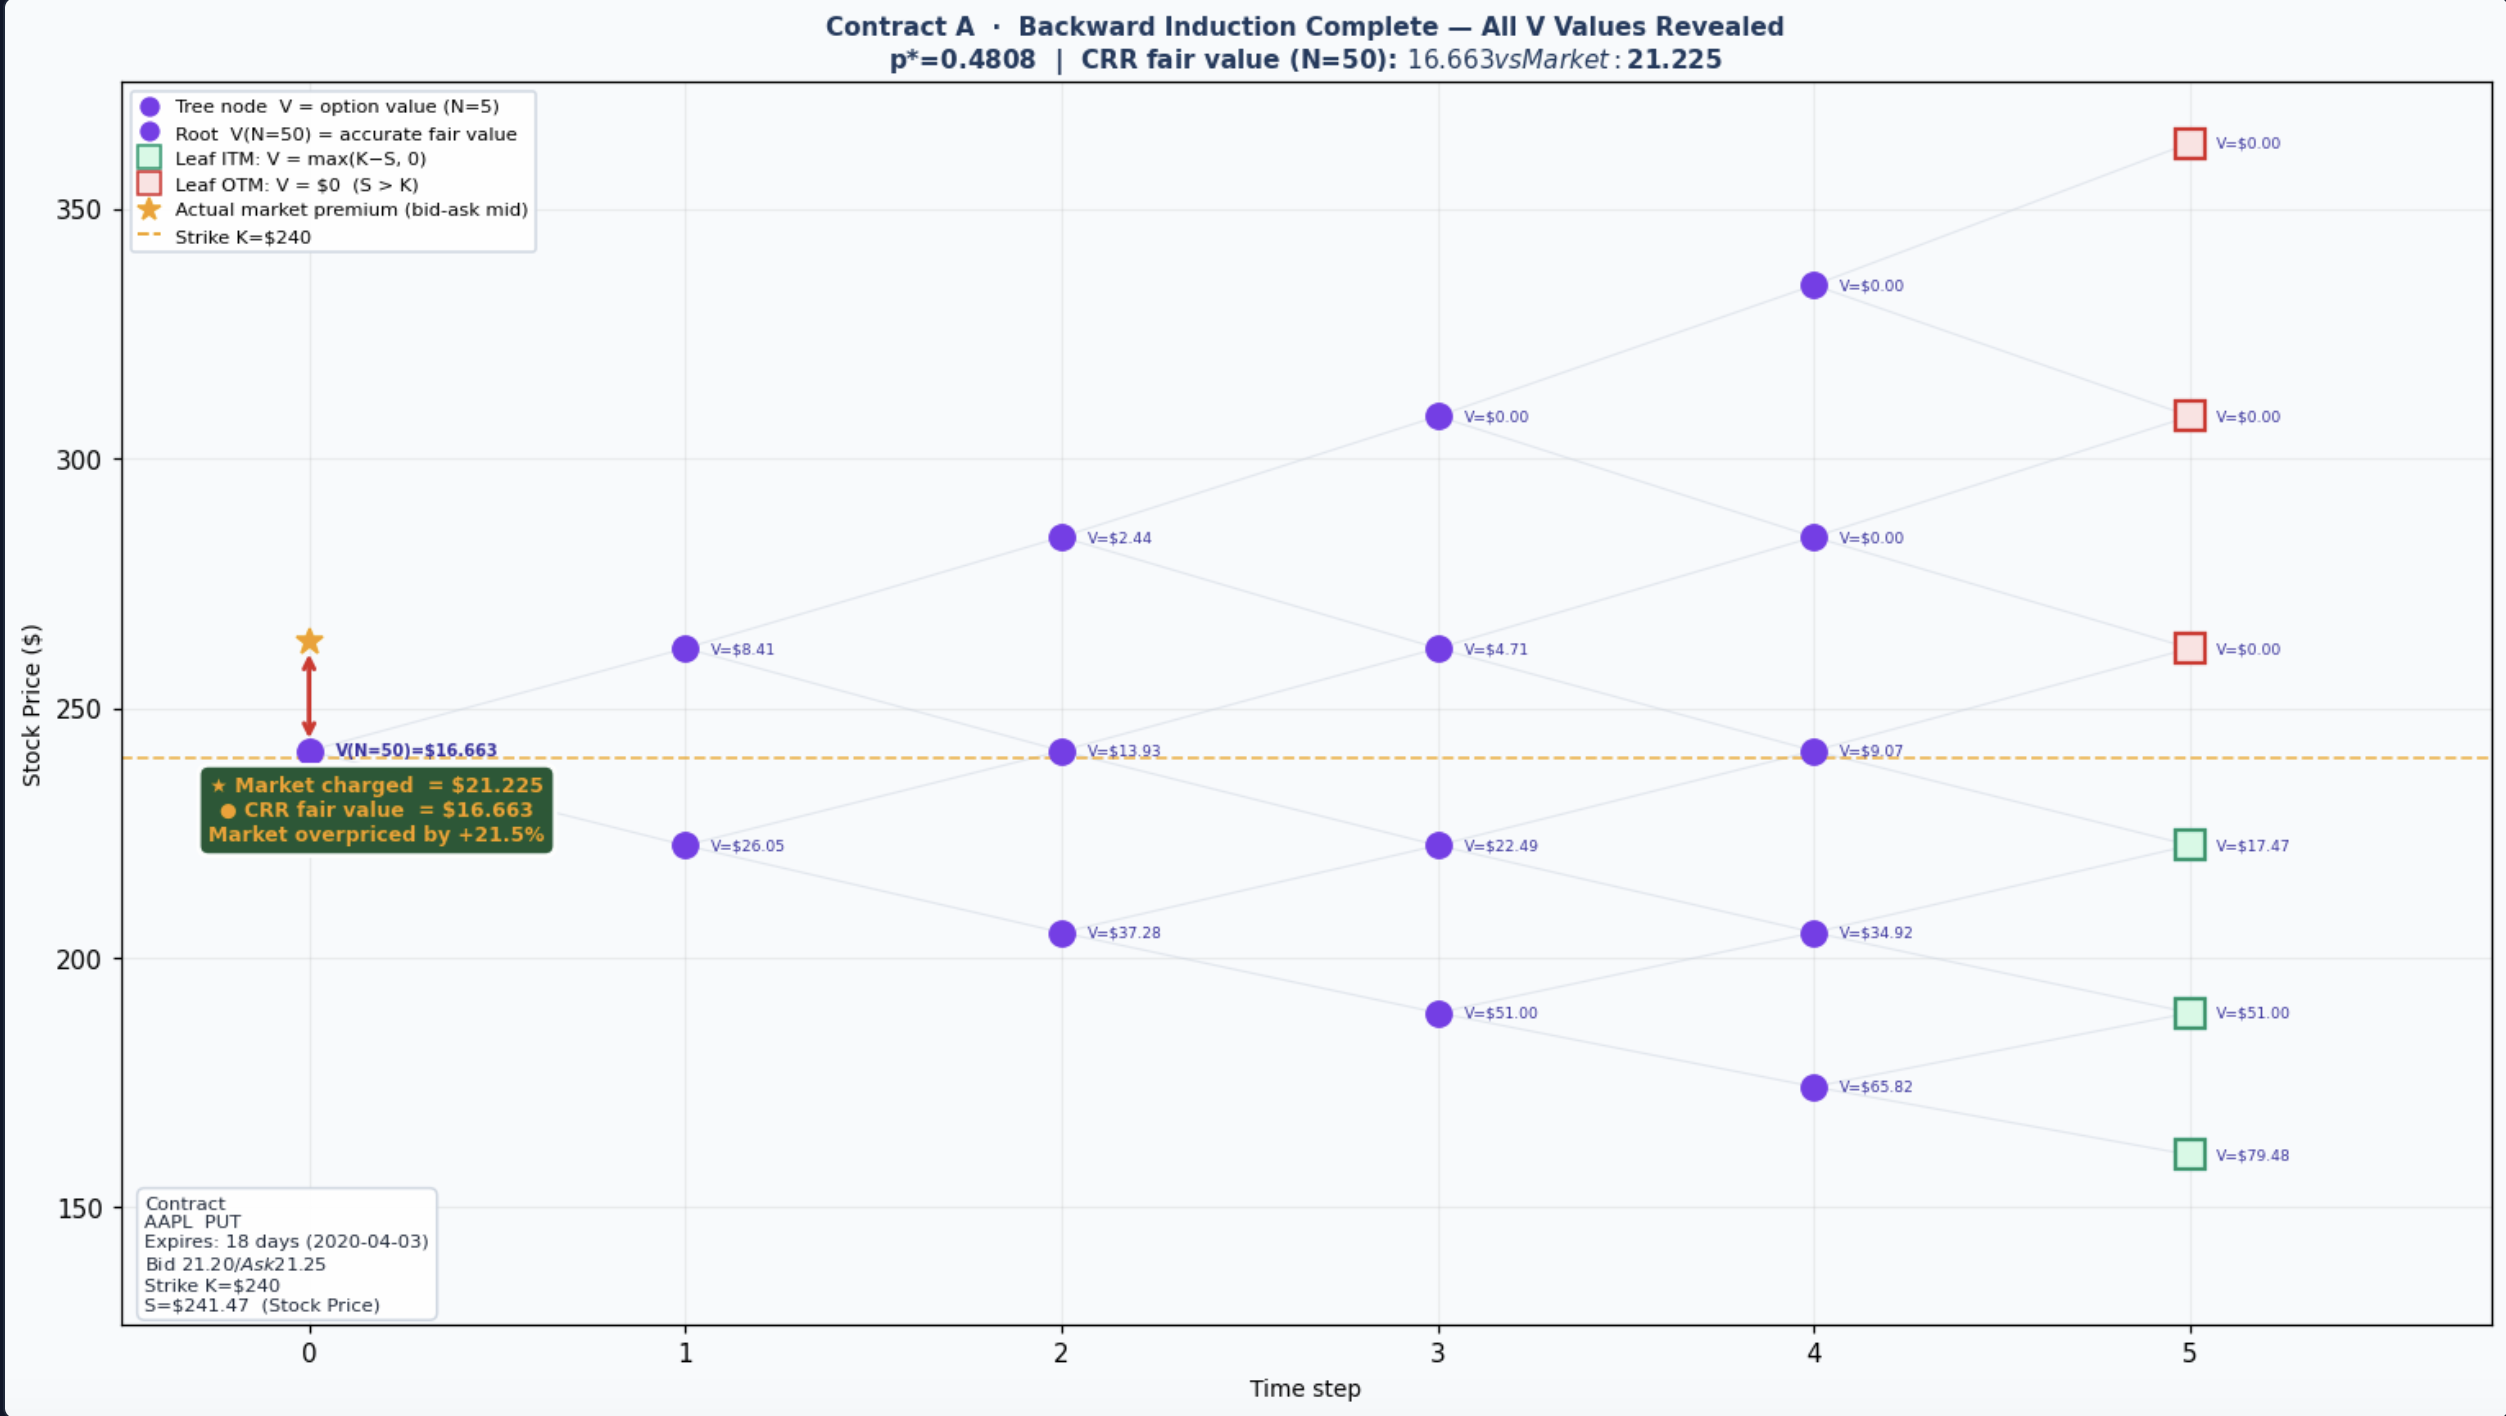
\includegraphics[width=0.62\linewidth,keepaspectratio]
    {Poster-Backward-Pass.png}
\end{center}
\end{posterblock}

\begin{posterblock}{Implementation \& Tools}
The entire pipeline is one command (\texttt{make run-all}) on any laptop
with Python 3.13. An interactive Streamlit application reproduces every
result end-to-end.

\vspace{0.4em}
\renewcommand{\arraystretch}{1.3}
\begin{tabular}{@{}p{0.32\linewidth}p{0.62\linewidth}@{}}
\toprule
\textbf{Component} & \textbf{Tools / Libraries} \\
\midrule
Language       & Python 3.13 \\
Modeling       & CRR (custom), XGBoost, scikit-learn \\
Data           & pandas, NumPy, yfinance \\
Visualization  & matplotlib, Streamlit \\
Deployment     & Streamlit (local), Poetry \\
Documentation  & LaTeX/Beamer, Markdown \\
Source control & Git, GitHub \\
\bottomrule
\end{tabular}
\end{posterblock}

% ──────────────────────────────────────────────────────────────────────────────
\columnbreak
%  RIGHT COLUMN
% ──────────────────────────────────────────────────────────────────────────────

\begin{posterblock}{Results}
\textbf{Contract A} (real AAPL put, herding regime):
$S=\$241.47$, $K=\$240$, DTE $=18$d. Both independent models
arrive at the same trade decision:

\vspace{0.4em}
\begin{center}
  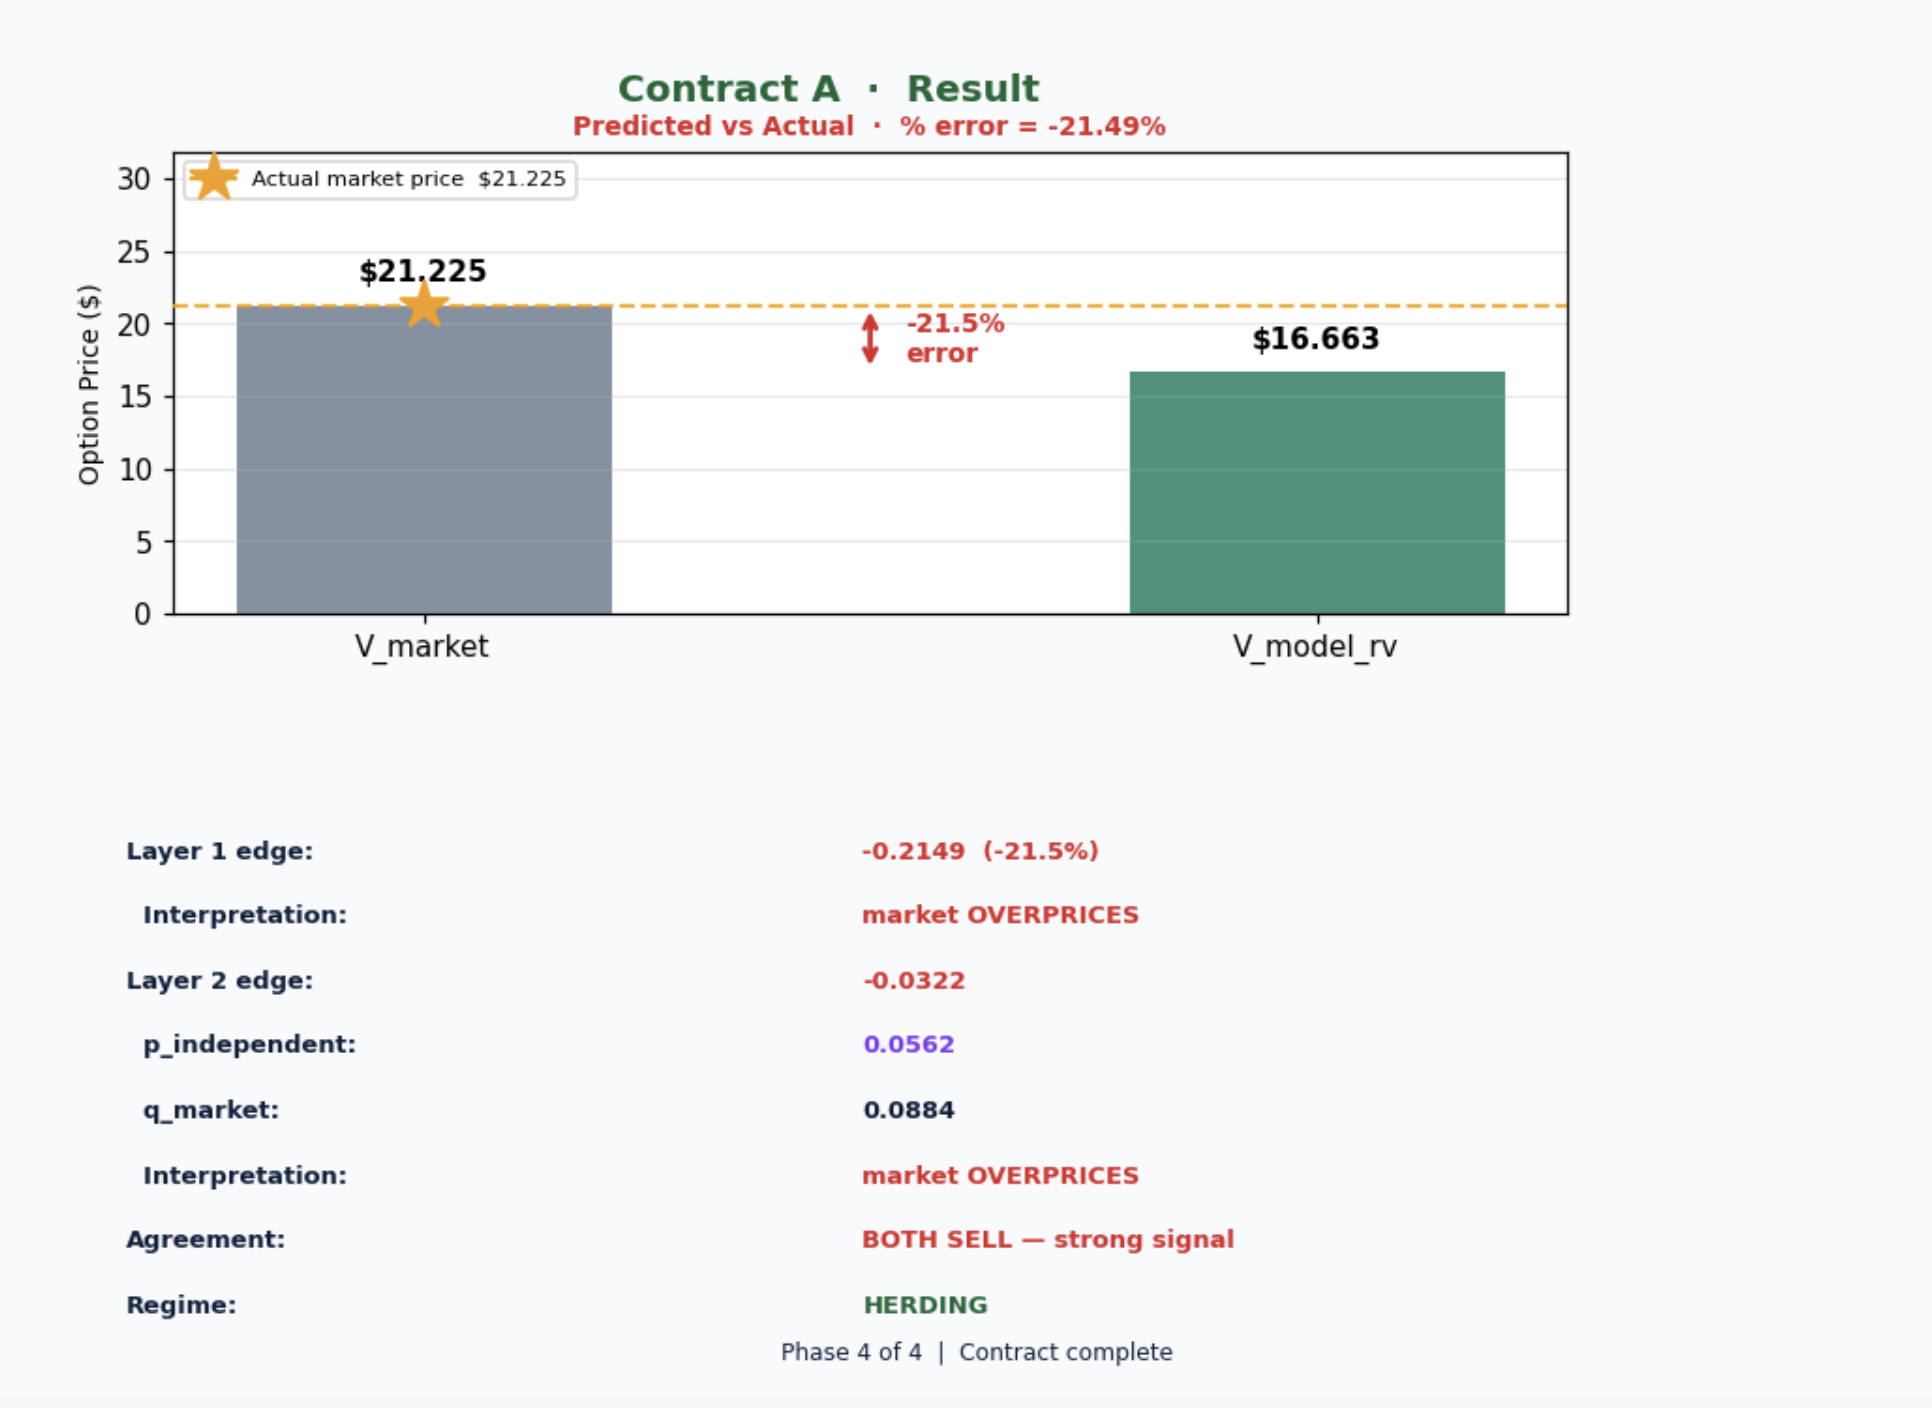
\includegraphics[width=0.72\linewidth,keepaspectratio]
    {Poster-Option-Pricing-Results.png}
\end{center}

\vspace{0.3em}
Layer 1 (CRR) edge $= -21.5\%$, Layer 2 (XGBoost) edge $= -3.2\%$:
\textbf{both layers say SELL} on this contract.

\vspace{0.6em}
\textbf{Performance summary} (101{,}535 AAPL contracts, walk-forward):

\vspace{0.3em}
\renewcommand{\arraystretch}{1.35}
\centering
\begin{tabular}{@{}lccc@{}}
\toprule
\textbf{Model} & \textbf{Brier} & \textbf{Hit rate} & \textbf{P\&L (\$)} \\
\midrule
Baseline (random)        & 0.250 & 50.0\%        & $0$         \\
Layer 1 CRR              & ---   & 63.0\%        & $+1.4$M     \\
Layer 2 XGBoost          & 0.211 & 66.5\%        & $+1.8$M     \\
\textbf{L1 $\cap$ L2 agree (Q3)} & --- & \textbf{76.5\%} & $+\mathbf{2.9}$M \\
\bottomrule
\end{tabular}
\RaggedRight

\vspace{0.6em}
\textbf{Cross-model agreement statistic:} Pearson correlation
coefficient $r = 0.413$ in herding regime ($n=217$,
$p = 2.4\times10^{-10}$); $r \approx 0$ in normal regime.
Max drawdown $<15\%$; \texttt{regime-conditioned} Kelly
(half-Normal, quarter-Herding) keeps risk bounded.
\end{posterblock}

\begin{posterblock}{Discussion \& Conclusions}
The central contribution is the \emph{cross-validation result}: two
\textbf{independent} models --- one mathematical (CRR no-arbitrage),
one empirical (XGBoost ML) --- detect the same mispricing direction
precisely in the regime behavioral finance theory predicts. Neither
layer is trained on the other; concurrent signals therefore come from
\emph{shared underlying reality}.

\vspace{0.5em}
\textbf{Key takeaways}
\begin{itemize}[leftmargin=1.4em,itemsep=4pt,topsep=4pt]
  \item Independent math + ML methods agree where the EMH literature
        says crowd bias is strongest (Fama, 1970; Samuelson
        macro-inefficiency).
  \item Kelly sizing converts the cross-validated edge into capital
        allocation with bounded drawdown.
  \item The framework's most valuable output is the \emph{no-trade}
        signal --- when CRR and XGBoost disagree, no position is taken.
  \item Reproducible: one \texttt{make run-all} regenerates every
        artifact end-to-end from raw data.
\end{itemize}

\vspace{0.3em}
\textbf{Limitations.} AAPL 2016--2020 is a single equity in a single
market cycle; CRR uses a flat IV per contract (no smile / skew);
backtest assumes mid-price fills with no transaction friction; regime
detection is backward-looking via IV/RV$_{30}$.

\vspace{0.3em}
\textbf{Future work.} Expand to SPY / QQQ / NDX options; integrate
LSTM volatility forecaster; live paper-trading via IBKR / Alpaca;
multi-leg spreads (vertical, calendar, iron condor) with joint Kelly
sizing.
\end{posterblock}

\begin{posterblock}{References}
\normalsize
\begin{enumerate}[leftmargin=1.6em,itemsep=4pt,topsep=4pt]
  \item Black, F. \& Scholes, M. (1973). The Pricing of Options and
        Corporate Liabilities. \emph{Journal of Political Economy} 81(3),
        637--654.
  \item Cox, J., Ross, S., \& Rubinstein, M. (1979). Option Pricing:
        A Simplified Approach. \emph{Journal of Financial Economics} 7(3),
        229--263.
  \item Fama, E.\,F. (1970). Efficient Capital Markets: A Review of
        Theory and Empirical Work. \emph{Journal of Finance} 25(2),
        383--417.
  \item Carr, P. \& Wu, L. (2009). Variance Risk Premiums.
        \emph{Review of Financial Studies} 22(3), 1311--1341.
  \item Kelly, J.\,L. (1956). A New Interpretation of Information Rate.
        \emph{Bell System Technical Journal} 35(4), 917--926.
  \item MacLean, L., Thorp, E.\,O. \& Ziemba, W. (2010). Good and Bad
        Properties of the Kelly Criterion. \emph{Quantitative Finance}
        10(1), 7--14.
\end{enumerate}
\end{posterblock}

\begin{posterblock}{Acknowledgments \& Contact}
The author thanks \textbf{Dr.~Pedro Albuquerque} for his guidance
throughout CS\,495, and the Bellevue College Computer Science program
for supporting this capstone project.

\vspace{0.6em}
\textbf{Contact:} \texttt{dewayne.dantzler@bellevuecollege.edu}\\
\textbf{Code / Repository:}
\texttt{github.com/dantzlerdc/CS495-Deep-Scholar}

\vspace{0.5em}
\begin{center}
\fbox{\qrcode[height=3.5cm]{https://github.com/dantzlerdc/CS495-Deep-Scholar}}
\\[0.3em]
\small\textit{Scan to open the full repository}
\end{center}
\end{posterblock}

\end{multicols}

% ══════════════════════════════════════════════════════════════════════════════
%  FOOTER BAND
% ══════════════════════════════════════════════════════════════════════════════
\vfill
\noindent
\begin{tikzpicture}
  \fill[BCBlue] (0,0) rectangle (\textwidth, 2cm);
  \fill[BCRed]  (0,2cm) rectangle (\textwidth, 2.25cm);
  \node[anchor=west] at (1cm, 1cm)
    {\color{white}\bfseries\LARGE CS\,495 -- Data Science Project Practicum};
  \node[anchor=east] at (\textwidth-1cm, 1cm)
    {\color{white}\LARGE Bellevue College \;\textbullet\; Spring 2026};
\end{tikzpicture}

\end{document}
